\begin{document}
%%%WILL UPDATE
The CD4007UBE is a model featuring four on board CMOS circuits tied together. The various circuits were constructed by utilizing these onboard CMOS circuits. The experimental results will be discussed as follows: the NMOS inverter, the CMOS inverter, the AND logic gate, the ring oscillator, and finally the astable multivibrator. 

\subsection{NMOS inverter}
The only change required by the NMOS inverter is that the 4.4k$\Omega$ resistor was switched to a 4.3k$\Omega$ resistor due to the lack of the availability of the 4.4k$\Omega$ resistor. The substitution of a 4.3k$\Omega$ in series with a 100$\Omega$ with 5\% tolerances would introduce too much error into the design. 
\newline

The VTC of the NMOS inverter is shown in Figure \ref{fig:VTCnmosexp}.

\begin{figure}[H]
    \centering
        \centering
        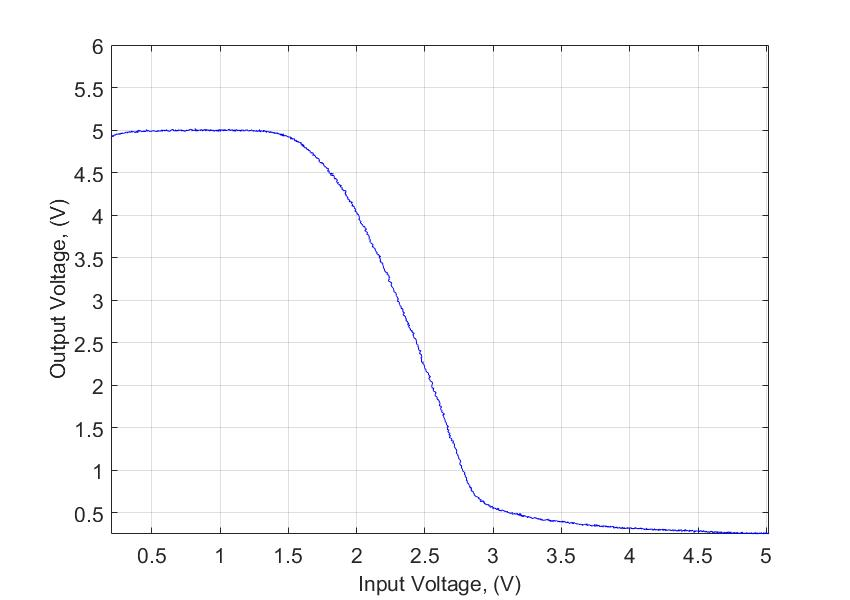
\includegraphics[scale = .35]{ExperimentalImplementation/VTC_NMOS_EXP.jpg}
        \caption{Experimental VTC NMOS}
        \label{fig:VTCnmosexp}
\end{figure} 
 The respective voltages for logic low versus logic high are shown. As expected from simulations, the low logic is not 0V, but instead a rather significant voltage. This accounts for the comparatively significant power consumption used by the NMOS inverter. The power consumption was found to be 5.8mW for logic high and 37$\mu$W for logic low. The output waveform is shown in Figure \ref{fig:voutnmos}
 
 
 \begin{figure}[H]
    \centering
    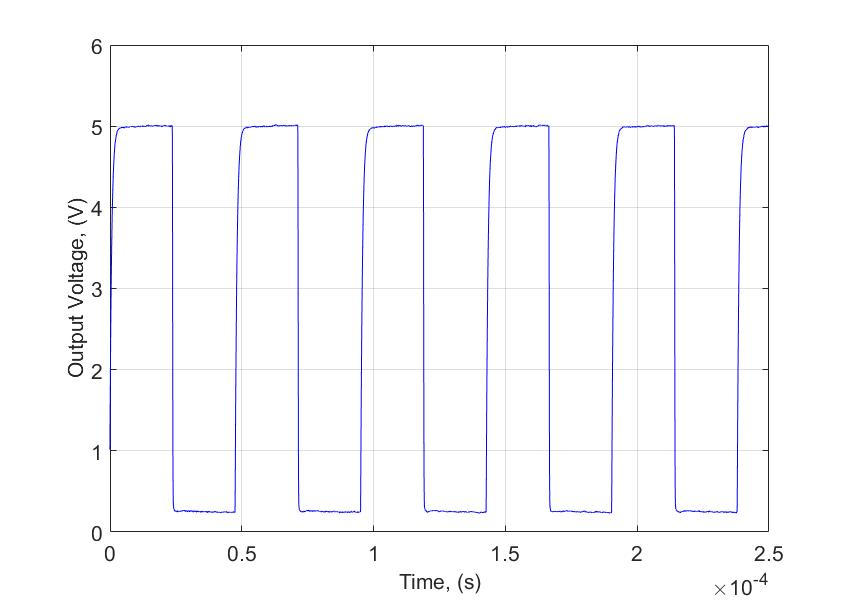
\includegraphics[width=.6\textwidth]{ExperimentalImplementation/nmos_waveform.jpg}
    \caption{Measured output of NMOS inverter}
    \label{fig:voutnmos}
\end{figure}
 
 The rise and fall times were found by the Digilent scope, the rise time was 11.4$\mu$s, and the fall time was 1.22$\mu$s. The experimental values for the NMOS inverter is shown in Table \ref{tab:expvalue}.

\begin{table}[H]
\centering
\caption{Experimental values}
\label{tab:expvalue}
\begin{tabular}{|l|l|}
\hline
Experiment Values & Results      \\ \hline
R                 & 4.3k$\Omega$ \\ \hline
Min Power         & 37$\mu$W     \\ \hline
Max Power         & 5.8mW        \\ \hline
V$_{max}$         & 5V           \\ \hline
V$_{min}$         & 400mV         \\ \hline
Rise Time         & 11.4$\mu$s       \\ \hline
Fall Time         & 1.22$\mu$s        \\ \hline
\end{tabular}
\end{table}


The experiment values that are expressed in Table \ref{tab:expvalue} are different than the simulated due to real world parasitic capacitance and limitations of the breadboard at higher frequencies.
The experimental results are as follows: the output voltage, which did not saturate; the frequency response, with a center frequency of 20.2kHz; and the bench test, where the specifications were met.

\subsection{CMOS inverter}
The only change required for implementation was that all three CMOS inverters were wired together in order to create three inverters in series as opposed to the only simulated two. The measurements were still taken from the output of the first stage.
The VTC from the first stage is shown in Figure \ref{fig:CMOSvtc}

\begin{figure}[H]
    \centering
    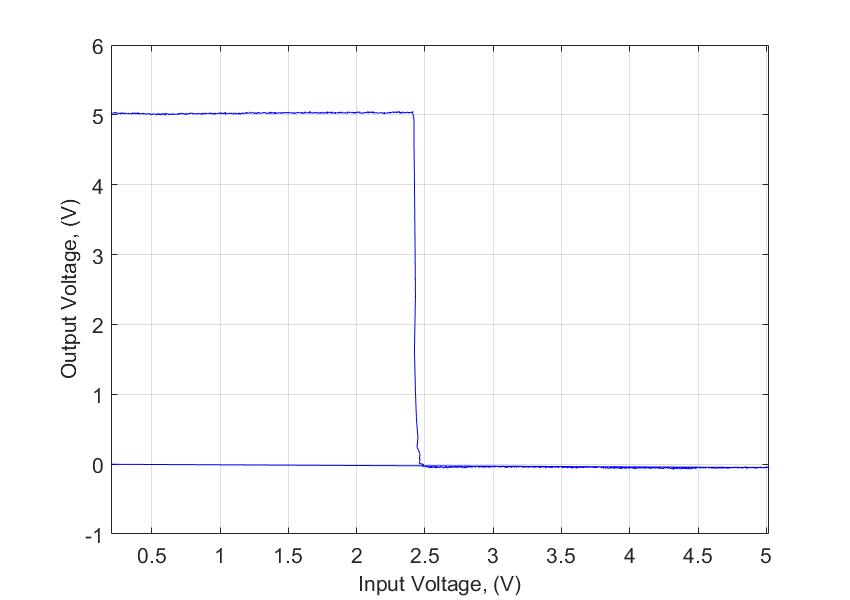
\includegraphics[width=.6\textwidth]{ExperimentalImplementation/CMOS_VTC_exp.jpg}
    \caption{Measured VTC of CMOS inverter}
    \label{fig:CMOSvtc}
\end{figure}

The VTC, as seen in Figure \ref{fig:CMOSvtc},  represents logic low as 0V, and improvement over the 400mV of the NMOS inverter. The CMOS inverter also features 0V$_{DC}$ power consumption opposed to the NMOS inverter. The output waveform for the CMOS is shown in Figure \ref{fig:CMOSout}.

\begin{figure}[H]
    \centering
    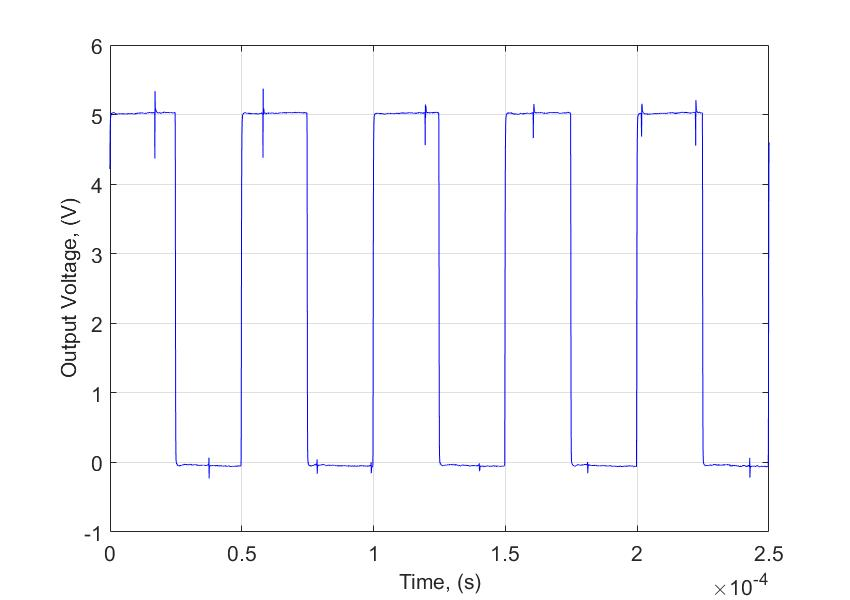
\includegraphics[width=.6\textwidth]{ExperimentalImplementation/cmos_waveform.jpg}
    \caption{Measured output of CMOS inverter}
    \label{fig:CMOSout}
\end{figure}

The subsequent rise and fall times were measured using the Digilent and were found to be 235ns for rise time and 177ns for the fall time. These are greater than those of the simulation, but is not unexpected due to parasitic capacitances and inductances from the jumper wires.


\subsection{AND gate}
The AND gate was created using all three CMOS circuits on the chip. A NAND gate was constructed using the first two on board CMOS circuits which were then inputed to a CMOS inverter. Figure \ref{fig:NANDpin} shows the pinout for an AND gate using the CD4007 IC.


\begin{figure}[H]
    \centering
    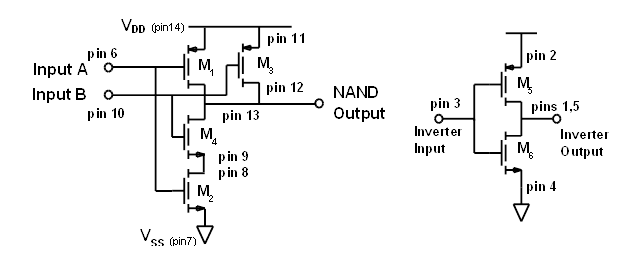
\includegraphics[width=.6\textwidth]{ExperimentalImplementation/NAND_pinout.png}
    \caption{Pinout for AND gate}
    \label{fig:NANDpin}
\end{figure}

The output from the NAND gate but before the inverter is expressed in Table \ref{tab:truthNAND}.

\begin{table}[H]
\centering
\caption{Truth Table: NAND}
\label{tab:truthNAND}
\begin{tabular}{|l|l|l|}
\hline
\multicolumn{2}{|l|}{Inputs} & Output \\ \hline
A             & B            & Z      \\ \hline
0             & 0            & 1      \\ \hline
0             & 1            & 1      \\ \hline
1             & 0            & 1      \\ \hline
1             & 1            & 0      \\ \hline
\end{tabular}
\end{table}

The inputs A and B were created by using the Digilent wave generator set to the DC setting, a logic 1 was 2.5V and logic 0 was 0V. The final output after the inverter is expressed in Table \ref{tab:truthAND}.

\begin{table}[H]
\centering
\caption{Truth Table: AND}
\label{tab:truthAND}
\begin{tabular}{|l|l|l|}
\hline
\multicolumn{2}{|l|}{Inputs} & Output \\ \hline
A             & B            & Z      \\ \hline
0             & 0            & 0      \\ \hline
0             & 1            & 0      \\ \hline
1             & 0            & 0      \\ \hline
1             & 1            & 1      \\ \hline
\end{tabular}
\end{table}

The time-domain graphs for these outputs are of little value, as they express simply a DC voltage at either 2.5V or 0V. 

\subsection{Ring oscillator}
The experimental oscillator required several changes. 8.2nF capacitors were the closest value available to the calculated 8nF. The circuit built with the 8.2nF operated at a frequency of 22.8kHz, which is not within specifications, that frequency is too far outside the bandwidth of the MFBP filter from the previous lab. An additional 4.7nF capacitor was added in parallel with the second stage of the oscillator, resulting in the final circuit is shown in Figure \ref{fig:expring}.

\begin{figure}[H]
    \centering
    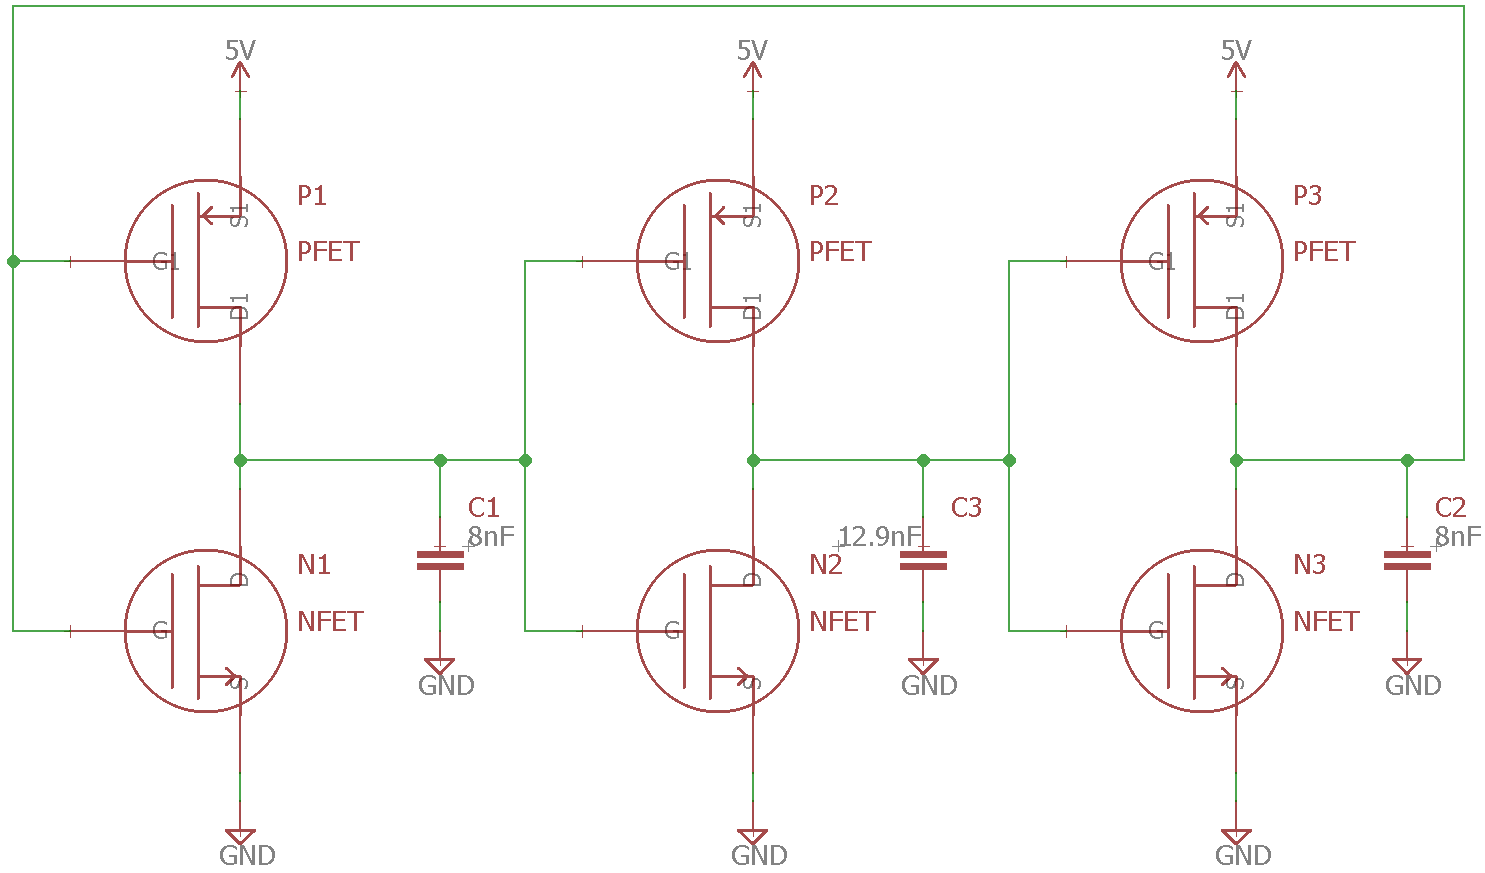
\includegraphics[width=.7\textwidth]{ExperimentalImplementation/RingOscillatorCMOSexp.png}
    \caption{Experimental ring oscillator circuit}
    \label{fig:expring}
\end{figure}

The transient analysis was performed on the circuit using the Digilent Scope function. The output waveform is shown in Figure \ref{fig:ringoutput}.

\begin{figure}[H]
    \centering
    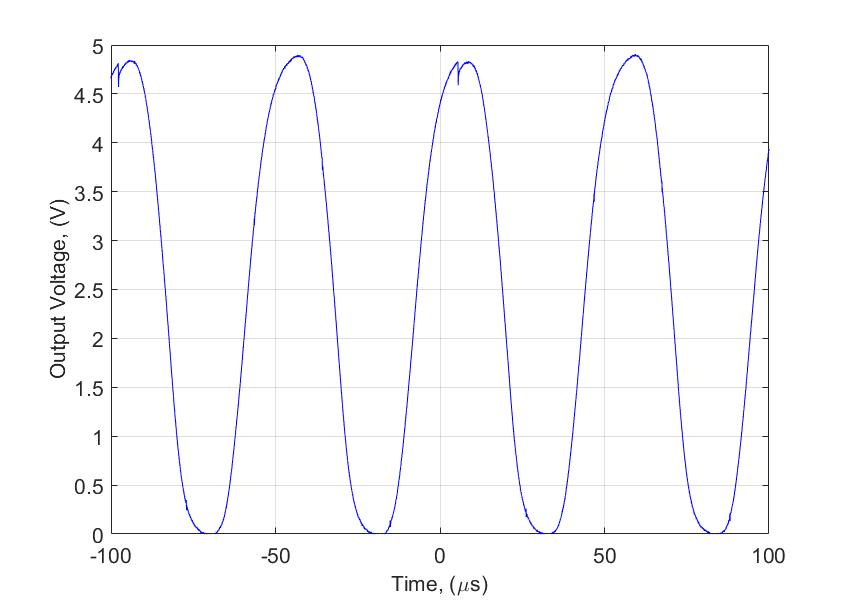
\includegraphics[width=.6\textwidth]{ExperimentalImplementation/ring_oscillator_output.jpg}
    \caption{Experimental transient analysis}
    \label{fig:ringoutput}
\end{figure}

The frequency was found to be 19.8kHz, a 51\% duty-cycle, with a 4.9V peak to peak amplitude. This frequency falls well within the bandwidth of the MFBP filter.


The final experimental results are summarized in Table \ref{tab:expfinal}.

\begin{table}[H]
\centering
\caption{Experimental results}
\label{tab:expfinal}
\begin{tabular}{|l|l|}
\hline
Value            & Experimental \\ \hline
Center Frequency & 19.8 kHz     \\ \hline
Duty-cycle       & 51\%      \\ \hline
Amplitude        & 4.9V     \\ \hline
\end{tabular}
\end{table}

The experimental results fall within the lab specifications outlined.



\end{document}